\documentclass{beamer}
\usefonttheme[onlymath]{serif}
\usepackage[T1]{fontenc}
\usepackage[utf8]{inputenc}
\usepackage[english]{babel}
\usepackage{amsmath}
\usepackage{amssymb}
\usepackage{amsthm}
\usepackage{gensymb}
\usepackage{parskip}
\usepackage{mathtools}
\usepackage{listings}
\usepackage{hyperref}
\usepackage{graphicx}
\usepackage{color}
\usepackage{enumerate}
\usepackage{tikz}
\usetikzlibrary{calc}
\usetikzlibrary{positioning}
\usetikzlibrary{angles}
\usetikzlibrary{shapes}
\usetikzlibrary{arrows}
\usepackage{verbatim}
\usepackage{multicol}
\usepackage{array}
\usepackage{minted}
\parskip 0pt


\DeclareMathOperator{\lcm}{lcm}
\newcommand\floor[1]{\left\lfloor#1\right\rfloor}
\newcommand\ceil[1]{\left\lceil#1\right\rceil}
\newcommand\abs[1]{\left|#1\right|}
\newcommand\p[1]{\left(#1\right)}
\newcommand\sqp[1]{\left[#1\right]}
\newcommand\cp[1]{\left\{#1\right\}}
\newcommand\norm[1]{\left\lVert#1\right\rVert}

\usetheme{metropolis}
\definecolor{dark yellow}{rgb} {0.6,0.6,0.0}
\definecolor{dark green}{rgb} {0.0,0.6,0.0}

\graphicspath{{myndir/}}

\title{Combinatorics}
\author{Atli FF}
\institute{\href{http://ru.is/td}{School of Computer Science} \\[2pt] \href{http://ru.is}{Reykjavík University}}
\titlegraphic{\hfill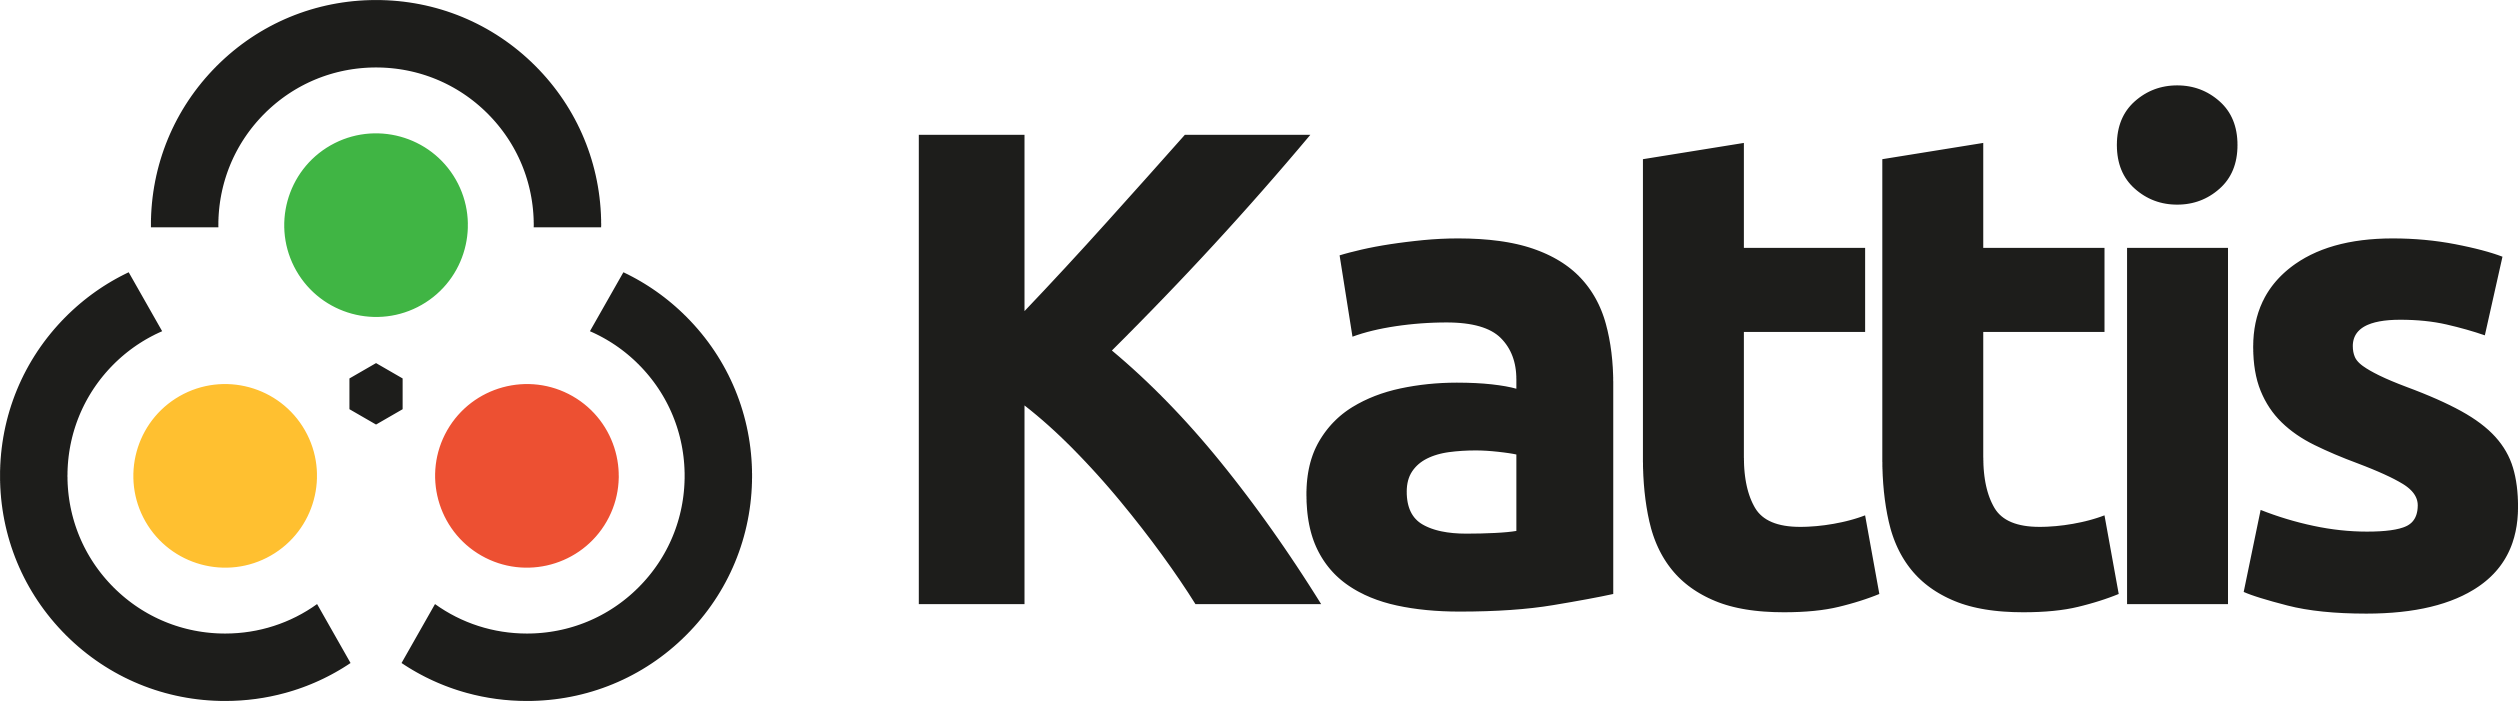
\includegraphics[height=0.6cm]{kattis}}

\begin{document}

\maketitle

\begin{frame}[plain]{Today's material}
    \vspace{22pt}
    \begin{itemize}
        \item Counting
        \item Combinatorics
        \item Game theory
        \item Probability
    \end{itemize}
\end{frame}

\section*{Combinatorics}

\begin{frame}[plain]
  \frametitle{Combinatorics}
  \vspace{30pt}
  Combinatorics is study of countable discrete structures.

  \onslide<2->
  \vspace{10pt}
  \emph{Generic enumeration problem: } We are given an infinite sequence of
  sets $A_1, A_2, \ldots A_n, \ldots$ which contain objects satisfying a set of
  properties. Determine 
  \[
    a_n \coloneqq \lvert A_n \rvert
  \]
  for general $n$.
\end{frame}

\begin{frame}[plain]{The two rules}

\begin{itemize}

\item If you have $n$ options, you can pick one in $n$ ways clearly.

\item If you can choose one of $n$ options \textbf{or} one of $m$ options then there are $n + m$ ways to do so.

\item If you can choose one of $n$ options \textbf{and} one of $m$ options then there are $nm$ ways to do so.

\item Most things can be derived from these two rules really.

\end{itemize}

\end{frame}

\begin{frame}[plain]
  \frametitle{Examples}
  \vspace{30pt}
  \begin{itemize}
    \item Factorial %, number of permutations on $n$ objects
      \[
        n! = 1\cdot 2 \cdot 3 \cdots n
      \]
    \item Binomial coefficient % Number ways to choose $k$ objects from $n$ objects
      \[
        \binom{n}{k} = \frac{n!}{k!(n-k)!}
      \]
      \onslide<2->
      Number of ways to choose $k$ objects from a set of $n$ objects, ignoring order.
  \end{itemize}
\end{frame}

\begin{frame}[plain]
  \frametitle{Binomial properties}
  \vspace{30pt}
  Properties
  \begin{itemize}
    \item \[
        \binom{n}{k} = \binom{n}{n-k}
    \]
    \item \[
        \binom{n}{0} = \binom{n}{n} = 1
      \]
    \item \[
        \binom{n}{k} = \binom{n-1}{k-1} + \binom{n-1}{k}
      \]
  \end{itemize}
\end{frame}

\begin{frame}[plain,fragile]
    \frametitle{Pascal triangle!}
  \begin{figure}
    \def\N{10}
    \tikz[x=0.75cm,y=0.5cm, 
      pascal node/.style={font=\footnotesize}, 
      row node/.style={font=\footnotesize, anchor=west, shift=(180:1)}]
      \path  
        \foreach \n in {0,...,\N} { 
          (-\N/2-1, -\n) node  [row node/.try]{}
            \foreach \k in {0,...,\n}{
              (-\n/2+\k,-\n) node [pascal node/.try] {%
    %            \pgfkeys{/pgf/fpu}%
    %            \pgfmathparse{round(\n!/(\k!*(\n-\k)!))}%
    %            \pgfmathfloattoint{\pgfmathresult}%
    %            \pgfmathresult%
                 $\binom{\n}{\k}$  
            }}};
  \end{figure}
\end{frame}

\begin{frame}[plain]
    \frametitle{Other useful identities}
  \begin{itemize}
    \item \[
        \sum_{k=0}^n \binom{n}{k} = 2^n
    \]
    \item \[
        \sum_{k=0}^n \binom{n}{k}^2 = \binom{2n}{n}
    \]
    \item The ``hockey stick sum'' \[
        \sum_{k=0}^{m} \binom{n+k}{k} = \binom{n+m+1}{m}
    \]
  \end{itemize}
\end{frame}

\begin{frame}[plain]
    \frametitle{Example}
    \vspace{20pt}
    How many rectangles can be formed on a $m\times n$ grid?

    \only<2-> {
        The rectangle is defined by covering some $x$-interval and some $y$-interval, we can choose these
        independently. If we have values $1, \dots, k$ and want to choose an interval, how can we do this?
    }

    \only<3-> {
        Well we want to choose $2$ out of $k$ values, without ordering since that's chosen by the values of the
        numbers. Thus this gives $\binom{k}{2}$ choices. Final answer is thus $\binom{n}{2}\binom{m}{2}$.
    }
\end{frame}

\begin{frame}[plain]
  \vspace{20pt}
  \frametitle{Multinomial}
  What if we have many objects with the same value?
  \begin{itemize}
    \onslide<2->
    \item Number of permutations on $n$ objects, where $n_i$ is the number of
      objects with the $i$-th value.(Multinomial)
      \[
        \binom{n}{n_1,n_2,\ldots,n_k} = \frac{n!}{n_1!n_2!\cdots n_k!}
      \]
    \onslide<3->
    \item Number of way to choose $k$ objects from a set of $n$ objects with, where each value can be chosen more than once.
      \[
        \binom{n + k - 1}{k} = \frac{(n + k - 1)!}{k!(n-1)!}
      \]
  \end{itemize}
\end{frame}

\begin{frame}[plain]
  \frametitle{Balls and boxes}
  \vspace{30pt}
  How many different ways can we divide $k$ identical balls into $n$ boxes?
  \begin{itemize}
    \onslide<2->
    \item Same as number of nonnegative solutions to
      \[
        x_1 + x_2 + \ldots + x_n = k
      \]
    \onslide<3->
    \item Let's imagine we have a bit string consisting only of $1$ of length $n+k-1$
      \[
        \underbrace{1\;1\;1\;1\;1\;1\;1\ldots1}_{n+k-1}
      \]
  \end{itemize}
\end{frame}

\begin{frame}[plain]
  \frametitle{Stars and bars}
  \vspace{20pt}
  \begin{itemize}
    \item Choose $n-1$ bits to be swapped for $0$
      \[
        %\underbrace{1\ldots1}_{x_1}0\underbrace{1\ldots1}_{x_2}0\ldots0\underbrace{1\ldots1}_{x_n}
        \only<1>{\,1\ldots1\,0\,1\ldots1\,0\ldots0\,1\ldots1}
        \only<2->{\underbrace{1\ldots1}_{x_1}0\underbrace{1\ldots1}_{x_2}0\ldots0\underbrace{1\ldots1}_{x_n}}
      \]
    \onslide<2->
    \item Then total number of $1$ will be $k$, each $1$ representing an each element, and separated into $n$ groups
    \onslide<3->
    \item Number of ways to choose the bits to swap
      \[
        \binom{n+k-1}{n-1} = \binom{n+k-1}{k}
      \]
  \end{itemize}
\end{frame}

\begin{frame}[plain,fragile]
  \frametitle{Example}
  \vspace{10pt}
  How many different lattice paths are there from $(0,0)$ to $(n,m)$?
  \vspace{-10pt}
      \vspace{10pt}
      \footnotesize
      \begin{itemize}
        \onslide<2->
        \item There is $1$ path to $(0,0)$
        \onslide<3->
        \item There is $1$ path to $(1,0)$ and $(0,1)$
        \onslide<4->
        \item Paths to $(1,1)$ is the sum of number of paths to $(0,1)$ and $(1,0)$.
        \only<5>{
        \item Number of paths to $(i,j)$ is the sum of the number of paths to $(i-1, j)$ and $(i,j-1)$.
        }
        \only<6->{
        \item Number of paths to $(i,j)$ is \[
            \binom{i+j}{i}
        \]
      }
      \end{itemize}
\end{frame}

\begin{frame}[plain]
  \frametitle{Dyck}
  What if we are not allowed to cross the main diagonal?
  \begin{columns}
    \begin{column}{.4\textwidth}
      \begin{figure}
        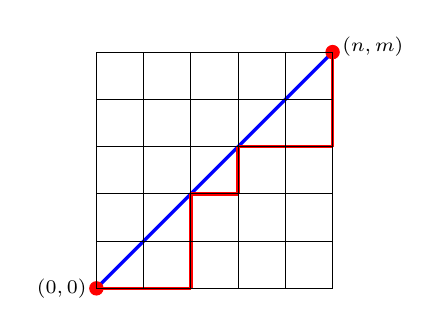
\begin{tikzpicture}[scale=0.6, bla node/.style={font=\scriptsize,draw=blue,text=blue,fill=blue}]
          \draw[blue,very thick] (0,0) -- (5,5);
          \draw[red,fill] (0,0) circle[radius=4pt];
          \draw[red,fill] (5,5) circle[radius=4pt];
          \draw (0,0) node[anchor=east] {\scriptsize $(0,0)$};
          \draw (5,5) node[anchor=west,yshift=2pt] {\scriptsize $(n,m)$};

          \onslide<2->{
          \draw[red, very thick] (0,0) -- (2,0);
          \draw[red, very thick] (2,0) -- (2,2);
          \draw[red, very thick] (2,2) -- (3,2);
          \draw[red, very thick] (3,2) -- (3,3);
          \draw[red, very thick] (3,3) -- (5,3);
          \draw[red, very thick] (5,3) -- (5,5);
          }
        \draw[step=1.0cm, thin] (0,0) grid (5,5);
        \end{tikzpicture}
      \end{figure}
    \end{column}
    \begin{column}{.6\textwidth}
      \begin{itemize}
        \onslide<2->
        \item The number of paths from $(0,0)$ to $(n,m)$
          \[
            C_n = \frac{1}{n+1}\binom{2n}{n}
          \]
        \onslide<3->
        \item $C_n$ are known as Catalan numbers.
        \item Many problems involve solutions given by the Catalan numbers.
      \end{itemize}
    \end{column}
  \end{columns}
\end{frame}

\begin{frame}[plain]
  \frametitle{More Catalan}
  \begin{itemize}
    \item Number of different ways $n+1$ factors can be completely parenthesized.
      \[
        ((ab)c)d\quad(a(bc))d\quad(ab)(cd)\quad a((bc)d)\quad a(b(cd))
      \]
    \onslide<2->
    \item Number of stack sortable permutations of length $n$.
    \onslide<3->
    \item Number of different triangulations convex polygon with $n+2$ sides
    \onslide<4->
    \item Number of full binary trees with $n+1$ leaves.
    \onslide<5->
    \item And a lot more.
  \end{itemize}
\end{frame}

\section*{Examples}

\begin{frame}[plain]
\frametitle{Working up to $\pi$}

\begin{itemize}

\item If we have $n$ options, but $m$ of them are forbidden, we are left with $n - m$ ways to choose.

\item This means if we have $n$ options and $m$ options, but $k$ of them are in common between them, that's $n + m - k$ different options. This can be rewritten as $\abs{A \cup B} = \abs{A} + \abs{B} - \abs{A \cap B}$.

\item We can keep going with this for larger numbers of sets, say options from $A$, $B$ and $C$. Then to know our total number of options we have to subtract what is in common. But if we do that thrice we will have removed what is in common between all three, which we need to add back.

\item In total this becomes
\begin{small}
\[\abs{A \cup B \cup C} = \abs{A} + \abs{B} + \abs{C} - \abs{A \cap B} - \abs{A \cap C} - \abs{B \cap C} + \abs{A \cap B \cap C}\]
\end{small}

\end{itemize}

\end{frame}

\begin{frame}[plain]
\frametitle{PIE}

\begin{itemize}

\item By generalizing this to $n$ sets using induction you can get an equation for the size of the union of $n$ sets $A_1, \dots, A_n$. This equation is usually called the principle of inclusion-exclusion, or PIE.

\[\abs{\bigcup_{i = 1}^n A_i} = \sum_{\substack{J \subseteq \{1,\dots,n\} \\ J \neq \varnothing}} (-1)^{\abs{J} - 1} \abs{\bigcap_{j \in J} A_j}\]

\end{itemize}

\end{frame}

\begin{frame}[plain]
\frametitle{Permutations}

\begin{itemize}

\item Let's look at permutations. Often it's convenient to denote them by a \textbf{bijective} function $\pi : [n] \rightarrow [n]$ where $[n] \coloneqq \{1, \dots, n\}$.

\item As mentioned before there are $n!$ permutations of $[n]$, but there's much more to it. A \textit{fixed point} of a permutation $\pi$ is an $x$ such that $\pi(x) = x$. Things we could consider regarding this include: how many permutations have no fixed points? Such permutation sare called derangements.

\item To count the number of derangements, we'll use a classic trick called counting the complement.

\item We know how many permutations there are, so we'll count how many permutations have \textit{some} fixed point and subtract that from the total.

\end{itemize}

\end{frame}

\begin{frame}[plain]
\frametitle{Fixed points}

\begin{itemize}

\item Let $A_i$ denote all permutations of $[n]$ where $i$ is a fixed point. Then we can permute everything but $i$ as usual, so $\abs{A_i} = (n - 1)!$. But if we want several values to be fixed, say everything in $J$, then we can use the same argument to get that there are $(n - \abs{J})!$ such permutations. Thus $\bigcap_{j \in J} A_j$ has $(n - \abs{J})!$ elements.

\item Thus we can now use PIE to count the size of $\bigcup_{j \in J} A_j$, which is what we want. We just have to keep in mind that the intersection of $k$ different $A_j$ will appear $\binom{n}{k}$ times. Thus

\[\sum_{i = 1}^n (-1)^{i - 1} \binom{n}{i} (n - i)! = n!\sum_{i = 1}^n (-1)^{i - 1}\frac{1}{i!}\]

\end{itemize}

\end{frame}

\begin{frame}[plain]
\frametitle{Derangement}

\begin{itemize}

\item Thus the number of derangements is just $n!$ minus this. We denote this by $!n$ and get

\[!n = n!\sum_{i = 0}^n \frac{(-1)^i}{i!}\]

\item A fun side effect of this is that $n!/!n$ very quickly approaches $e$ as $n$ grows.

\end{itemize}

\end{frame}

\begin{frame}[plain]
\frametitle{Permutations and sign}

\begin{itemize}

\item Permutations of $[n]$ have a whole lot more interesting combinatorial properties, but the two that appear the most in these kinds of problems are sign and inversion number.

\item Note that if $\sigma$ is a permutation we can look at $x, \sigma(x), \sigma(\sigma(x)), \dots$. Since $[n]$ is finite, this will eventually loop and we get a cycle in the permutation.

\item By considering what cycle each element belongs to, we can factor permutations into cycles. Thus we get a cycle form of permuations, so we can write for example $(x y z)(a b)(t)$ to denote $\sigma(x) = y$, $\sigma(y) = z$, $\sigma(z) = x$, $\sigma(a) = b$, $\sigma(b) = a$ and $\sigma(t) = t$. Note that the contents of the parentheses are disjoint.

\end{itemize}

\end{frame}

\begin{frame}[plain]
\frametitle{Sign}

\begin{itemize}

\item Furthermore we can rewrite $(a b c \dots x)$ as $(a b)(a c)\dots(a x)$ so all permutations can be written as a sequence of swaps. It can be proved that the parity of the number of swaps is fixed for a given permutation. So we call this parity its \textit{sign}.

\item We denote this by $\operatorname{sgn}(\pi)$ and make it $1$ when the number of swaps is even and $-1$ when the number of swaps is odd. Then we get that $\operatorname{sgn}(\pi_1 \circ \pi_2) = \operatorname{sgn}(\pi_1)\operatorname{sgn}(\pi_2)$ and $\operatorname{sgn}(\operatorname{id}) = 1$. This also means that $\operatorname{sgn}(\pi^{-1}) = \operatorname{sgn}(\pi)$.

\end{itemize}

\end{frame}

\begin{frame}[plain]
\frametitle{Inversions}

\begin{itemize}

\item Take $i, j \in [n]$. The ordered pair $(i, j)$ is called an \textit{inversion} of $\pi$ if $i < j$ but $\pi(i) > \pi(j)$.

\item The inversion number of $\pi$ is then the number of such swaps. 

\item But how can this be calculated efficiently?

\item One is to use segment trees, but another is to use mergesort and count how many inversions get fixed as you go.

\end{itemize}

\end{frame}

\begin{frame}[fragile, plain]
\frametitle{Invnum - Mergesort version}

\begin{small}
\begin{minted}{cpp}
ll merge(vi& v, vi& l, vi& r) {
  ll i = 0, j = 0, cnt = 0;
  while(i < l.size() || j < r.size()) {
    if(i == l.size()) v[i + j] = r[j], ++j;
    else if(j == r.size()) v[i + j] = l[i], ++i;
    else if(l[i] <= r[j]) v[i + j] = l[i], ++i;
    else v[i + j] = r[j], cnt += l.size() - i, ++j;
  } return cnt; }

ll invnum(vi &v) { if(v.size() < 2) return 0;
  int m = v.size() / 2; vi l(m), r(v.size() - m);
  copy(v.begin(), v.begin() + m, l.begin());
  copy(v.begin() + m, v.end(), r.begin());
  return invnum(l) + invnum(r) + merge(v, l, r); }
\end{minted}
\end{small}

\end{frame}

\begin{frame}[plain]
\frametitle{A counting problem}

\begin{itemize}

\item Let us consider an example from Kattis of a harder counting problem. We get $1 \leq n \leq 1000$ and $1 \leq c \leq 10000$ and want to find the number of permutations of $n$ elements with $c$ inversions. The answer should be returned modulo $10^9 + 7$.

\item Where do we start?

\item Can we solve the problem for $n, c$ in terms of smaller values?

\end{itemize}

\end{frame}

\begin{frame}[plain]
    \frametitle{Subdivision}

\begin{itemize}

\begin{small}
\item Denote the answer for $n, c$ by $f(n, c)$ and let us write our permutation as a list $\pi(1), \dots, \pi(n)$. We can make a permutation of $n + 1$ elements by adding $n + 1$ to this list. If we add it at location $k$ (and shift what's right of it) we add $n - k + 1$ inversions.

\item We can also do this backwards, starting with a permutation on $n$ elements and removing $n$. Let us consider permutations on $n$ lements with $c$ inversions and the value $n$ is $t$-th last in the list.

\item Then if we remove $n$ we fix $t - 1$ inversions, so we end up with a permutation on $n - 1$ elements with $c - t + 1$ inversions. Thus for this particular $t$ we get $f(n - 1, c - t + 1)$. By considering all $t$ we get:

\[f(n, c) = \sum_{i = 0}^{\min(c, n - 1)} f(n - 1, c - i)\]
\end{small}
\end{itemize}

\end{frame}

\begin{frame}[plain]
\frametitle{Dynamic programming}

\begin{itemize}

\item Now we have a recursive formula in terms of $(n, c)$, so we can use dynamic programming! But the time complexity is $\mathcal{O}(nc^2)$ because there are $nc$ states and each takes $c$ time to calculate.

\item We use the same trick as two days ago, we precalculate the sum so each value will only take constant time. For this we need bottom-up dynamic programming. So we define $p(n, c)$ as

\[p(n, c) = \sum_{i = 0}^c f(n, i)\]

\item Then we can update both $p$ and $f$ in constant time and solve the problem in $\mathcal{O}(nc)$ which is good enough!

\end{itemize}

\end{frame}

\begin{frame}[fragile, plain]
\frametitle{The code}

\begin{tiny}
\begin{minted}{cpp}
#include<bits/stdc++.h>
using namespace std;
const int mod = 1e9 + 7;

int n, c;
int dp[1005][10005];
int pr[1005][10005];

int main() {
    cin >> n >> c;
    if(c == 0) {
        cout << "1\n";
        return 0;
    }
    for(int i = 0; i <= c; ++i) dp[0][i] = 0;
    for(int i = 0; i < n; ++i) dp[i][0] = 1;
    for(int i = 1; i < n; ++i) {
        pr[i - 1][0] = dp[i - 1][0];
        for(int j = 1; j <= c; ++j) {
            pr[i - 1][j] = (pr[i - 1][j - 1] + dp[i - 1][j]) % mod;
        }
        for(int j = 1; j <= c; ++j) {
            dp[i][j] = pr[i - 1][j];
            if(j >= i + 1) {
                dp[i][j] -= pr[i - 1][j - i - 1];
                dp[i][j] = (dp[i][j] % mod + mod) % mod;
            }
        }
    }
    cout << dp[n - 1][c] << '\n'; }
\end{minted}
\end{tiny}

\end{frame}

\section*{Combinatorial equations}

\begin{frame}[plain]
\frametitle{Linear recurrences}

\begin{itemize}

\item Let us define a linear recurrence. We say a sequence of numbers follows a linear recurrence if they are defined using some initial values and then the subsequent values being defined by a linear equation of the form
\[a_n = \lambda_1 a_{n - 1} + \lambda_2 a_{n - 2} + \dots + \lambda_k a_{n - k} + \lambda\]
with the $\lambda_i$s constant. $k$ is said to be the degree of the recurrence relation.

\item An example of this is the fibonacci numbers, where $\lambda_1 = \lambda_2 = 1$, $\lambda = 0$ and $a_1 = a_2 = 1$.

\end{itemize}

\end{frame}

\begin{frame}[plain]
    \frametitle{Calculating a sequence}

\begin{itemize}

\item The trick is that using matrices we can calculate values in these sequences very fast. We can get the $n$-th number in $\mathcal{O}(k^3 \log(n))$ time. Since $k$ is usually very small, almost always $< 10$, this is quite fast. For example for fibonacci we have $k = 2$. The trick is the following equation:

\end{itemize}

\[
\p{\begin{matrix}
\lambda_1 & \lambda_2 & \cdots & \lambda_{k-1} & \lambda_k & \lambda \\
1 & 0 & \cdots & 0 & 0 & 0 \\
0 & 1 & \cdots & 0 & 0 & 0 \\
\vdots & \vdots & \ddots & \vdots & \vdots & \vdots \\
0 & 0 & \cdots & 1 & 0 & 0 \\
0 & 0 & \cdots & 0 & 0 & 1 \\
\end{matrix}}^n
\p{\begin{matrix}
a_k \\ a_{k - 1} \\ \vdots \\ a_2 \\ a_1 \\ 1 \\
\end{matrix}}
=
\p{\begin{matrix}
a_{n + k} \\ a_{n + k - 1} \\ \vdots \\ a_{n + 2} \\ a_{n + 1} \\ 1 \\
\end{matrix}}
\]

\end{frame}

\begin{frame}[plain]
\frametitle{Linear recurrence}

\begin{itemize}

\item So for example we can calculate the fibonacci numbers using:
\[\p{\begin{matrix}1 & 1\\1 & 0\end{matrix}}^n\p{\begin{matrix}1\\1\\\end{matrix}}\]

\item We omitted one row there since $\lambda = 0$. But similarly if $a_1 = 1, a_2 = 2$ and $a_n = 3a_{n-1} - a_{n - 2} + 6$ the corresponding calculation would be
\[\p{\begin{matrix}3 & -1 & 6\\1 & 0 & 0\\0 & 0 & 1\\\end{matrix}}^n\p{\begin{matrix}2\\1\\1\\\end{matrix}}\]

\end{itemize}

\section*{Probability}

\end{frame}
\begin{frame}[plain]
\frametitle{Probability theory}

\begin{itemize}

\item We will now briefly talk about probabilities.

\item Some problems use probabilities, but only really on a surface level so we won't delve deep.

\item Sometimes there are slightly more involved problems about markov chains and the like, but we won't go much into that here.

\item We won't formally define probabilities, measures, distributions and the like here. If you want to learn that take a probabilistics course.

\end{itemize}

\end{frame}

\begin{frame}[plain]
\frametitle{Discrete basics}

\begin{itemize}

\item In these problems we consider only discrete probabilities.

\item Then there are finitely (or at least countably) many options that can happen, $x_1, \dots, x_n$, and each of those has some probability $0 \leq P(x_i) \leq 1$ of occurring, such that $\sum P(x_i) = 1$. An \textbf{event} $X$ is then a set of such outcomes $x_i$.

\item If the $x_i$ correspond to numbers we can speak of expected values. $E[X]$ and is calculated using $E[X] = \sum x_i P(x_i)$.

\item The most important property of expected values is that it's linear. That is to say if we have some distributions $X$ and $Y$ and $a$ is some number, then $E[X + Y] = E[X] + E[Y]$ and $E[aX] = aE[X]$.

\end{itemize}

\end{frame}

\section*{Game theory}

\begin{frame}[plain]
\frametitle{Game theory}

\begin{itemize}

\item Game theory is the theory on games. The games we will consider are between players who always play perfectly and there is no hidden information (cards on hand or something).

\item The games are defined by states and what states can be reached from each of them. This means that for each state there is some set of legal moves. Some states will also be losing states, for tic-tac-toe this would for example be states where the opponent has three in a row.

\item For these kinds of games that only allow a finite number of moves we can work backwards to find out whether states are going to lead to a loss or to a win.

\end{itemize}

\end{frame}

\begin{frame}[plain]
    \frametitle{Working backwards}

\begin{itemize}

\item We start by collecting all end states (i.e. states where the game is over, either due to a tie or one player winning).
\item Then we recursively consider states. For all reachable states you pick the best one. If one of those is a losing position for the opponent then you choose that and your current state is a winning one. If none of them are losing states for the opponent you try to pick one that forces a tie. If neither are possible the current state is a losing one.

\item Let us consider an example.

\end{itemize}

\end{frame}

\begin{frame}[plain]
    \frametitle{Simple game}

\begin{itemize}

\item Let us consider a game where we start with $n$ stones in a pile. Two players take turns removing either one or two stones from the pile. The player taking the last stone wins. For what $n$ will $A$ win and for what $n$ will $B$ win if they play perfectly?

\item Well, if there are no stones left and it's your turn, you lose. Thus $0$ is a losing state.

\item If there are one or two stones left you can take the rest, so $1$ and $2$ are winning states.

\item If there are three left, then no matter whether you take one or two stones you put the opponent in a winning state, so $3$ is a losing state.

\end{itemize}

\end{frame}

\begin{frame}[plain]
    \frametitle{Simple game ctd.}

\begin{itemize}

\item You can continue like this and use induction to show that $n$ is a losing state iff $n = 0 \ (mod \ 3)$.

\item Since $A$ starts we thus get that $A$ loses iff the starting number of stones is a multiple of three.

\end{itemize}

\end{frame}

\begin{frame}[plain]
    \frametitle{Harder game}

\begin{itemize}

\item Let us consider another game with $n$ piles, each with $k_1, \dots, k_k$ stones. A player may now take as many stones as they wish, but only from one of the piles at a time. The one taking the last stone wins. This is a famous game theory game called nim.

\item It's much harder to see a winning strategy here, but there is a trick to it. The trick is to make sure that after your move $k_1 \oplus \dots \oplus k_n = 0$ where $\oplus$ is the XOR operation. But why might that be?

\item Well, $0$ is a losing state, so if $k_1 \oplus \dots \oplus k_n = 0$ after each of your moves and $k_1 \oplus \dots \oplus k_n \neq 0$ when it's your turn, surely you'll win. The reason we use $\oplus$ is that if this value is zero at the start of your turn, there is no way to keep it at zero.

\end{itemize}

\end{frame}

\begin{frame}[plain]
\frametitle{Xorsum}

\begin{itemize}

\item But how do we make sure it's zero after our move? We will have to assume it's not already $0$.

\item Let the xor-sum be $X$. Then we look at $X \oplus k_i$ for each $i$. Since $\oplus$ is associative and xor-ing twice cancels out, this will be the xor-sum of all piles but $k_i$. Thus there must be some pile such that $X \oplus k_j < k_j$ since $X \neq 0$. Thus we take $k_j - (X \oplus k_j) > 0$ stones from pile $j$, making the xor-sum $0$ after our move.

\item In the same vein if $X$ starts as zero, then no matter what move we make it won't be zero afterwards. Thus a state is a losing state iff $k_1 \oplus \dots \oplus k_n = 0$.

\end{itemize}

\end{frame}

\begin{frame}[plain]
    \frametitle{Grundy-Sprague}

\begin{itemize}

\item We will take a look at a theorem we won't prove. It's called the Grundy-Sprague theorem.

\item Let us have a game with no hidden information, no ties, both players make the same kinds of moves and one that is always over in a finite number of moves, ending when a player can't make any moves.

\item For any such game we can define a Grundy number for every state.

\end{itemize}

\end{frame}

\begin{frame}[plain]
    \frametitle{Grundy-numbers}

\begin{itemize}

\item We start by giving all ending states which lose the Grundy number $0$ (for example for nim this would be when all piles are empty).

\item We then define $\operatorname{mex}$. It stands for minimum excluded value. It takes a set of numbers and returns the smallest non-negative integer not in the set. We then let the Grunndy number of a state be the $\operatorname{mex}$ of all Grundy-numbers of states we can reach.

\item Then a state is a losing one iff the Grundy-number is zero. But this isn't the most useful part of the Grundy number.

\end{itemize}

\end{frame}

\begin{frame}[plain]
\frametitle{Grundy-Sprague}

\begin{itemize}

\item Imagine we have $k$ games going on in parallel, with a player only allowed to make a move in one of them on their turn. The player loses once they can't make a move in any of them.

\item Then the Grundy-Sprague theorem says that the Grundy number of a state in this game is the xor-sum of the Grundy numbers of the individual states in the games. Thus the position is a losing one iff the xor-sum of the Grundy numbers is $0$.

\end{itemize}

\end{frame}



\end{document}

